% LaTeX Article Template - using defaults
\documentclass[9pt,twoside]{exam}
%\textheight    23cm
%\textwidth     17.cm
%\oddsidemargin   .1cm
%\evensidemargin  .1cm
%\topmargin -0.9cm
%\parskip 3pt
%\pagestyle{myheadings}

\usepackage[english]{babel}
\usepackage{graphicx}
%\usepackage{showkeys}
\usepackage{datetime}
\usepackage[applemac]{inputenc}
\usepackage{amssymb,amsmath}
\usepackage[T1]{fontenc}
\usepackage{caption}
\usepackage{subcaption}
\usepackage{hyperref}
\usepackage{graphicx}
\usepackage[absolute]{textpos}
\usepackage{anyfontsize}
\usepackage{t1enc}
\usepackage[usenames, dvipsnames]{color}
\usepackage{lipsum}
\usepackage{tcolorbox}
\usepackage{pdfpages}
\usepackage{float}
\usepackage{pgfplots}
\pgfplotsset{width=10cm,compat=1.9}


% A nice serif font, but no the prescribed nonfree ITC stone
\usepackage[oldstylenums]{kpfonts}
\usepackage[T1]{fontenc}
%\usepackage{fancyhdr}
\definecolor{mygray1}{RGB}{128, 128, 128}
\definecolor{mygray2}{RGB}{77, 77, 77}
% No paragraph indentation
\pagestyle{empty}
\newcommand{\bigbar}{\rule[0ex]{0.41pt}{.75in}} 

\newcommand{\R}{\ensuremath{\mathbb R}}


\begin{document}
%%%%%%%%%%%%%%%%%%%%%%%%%%%%%%%%%%%%%%%%%%%
%%%%%%%%%%%%%%%%%%%%%%%%%%%%%%%%%%%%%%%%%%%
%%%%                       COVER PAGE begins                         %%%%%%%%%%%%%
%%%%%%%%%%%%%%%%%%%%%%%%%%%%%%%%%%%%%%%%%%%
%%%%%%%%%%%%%%%%%%%%%%%%%%%%%%%%%%%%%%%%%%%
%\begin{coverpages}
\title{\begin{tcolorbox} \begin{center}{CS 470\\ 
\vspace{0.5cm}
Data Mining\\
\vspace{0.5cm}
Homework 5\\
 } \end{center}
 \end{tcolorbox}}
% \vspace{2cm}
 \author{ 
 Jason Ji \\\\
Collaborations: Didn't collaborate with any other students.\\ Translated the code of minHash from python to Java, original code is linked here: \\https://github.com/chrisjmccormick/MinHash}
 \date{  }
 \maketitle
\pagestyle{myheadings}
\thispagestyle{plain}
\markboth{\; \hrulefill\;Homework 5 -  CS 470}{\; Homework 5 -  CS 470 \hrulefill\; }
\vspace{-0.5cm}



%%%%%%%%%%%%%%%%%%%%%%%%%%%%%%%%%%%%%%%%%%%
%%%%%%%%%%%%%%%%%%%%%%%%%%%%%%%%%%%%%%%%%%%
%%%%                       COVER PAGE ends                            %%%%%%%%%%%%%
%%%%%%%%%%%%%%%%%%%%%%%%%%%%%%%%%%%%%%%%%%%
%%%%%%%%%%%%%%%%%%%%%%%%%%%%%%%%%%%%




\newcommand{\bi}{\mathbf{i}}
\newcommand{\bbb}{\mathbf{b}}



\section*{Test Cases Description}

The data sets used in this assignment are articles\_100/1000/2500/10000.train, which represent a certain number of articles. Specifically, each line of the data represents an article with the article id followed by its content. Among these articles, some are plagiarisms of each other (where they have been just slightly modified). These near-duplicates are specified in articles\_100/1000/2500/10000.truth. An example of an article is shown below:
\\\\
t980 A man was shot dead and fifteen others injured when Zambian policemen clashed with citizens rioting in protest against alleged ritual murders by a local businessman, police said Monday. U.S. President George W. Bush expressed confidence on Monday about passing an immigration bill and said a Senate vote of no-confidence in Alberto Gonzales would have no bearing on his service as attorney general. French President Nicolas Sarkozy announced Tuesday in Washington that he would visit China later this month, joined by his wife, Carla Bruni-Sarkozy. These columns for release Tuesday, April 2, 2002 are moving today to clients of the New York Times News Service. Media and entertainment giant Viacom Inc. said Wednesday it may split into two divisions with one focussing on "growth" and the other, more traditional arm, aiming for "value". I don't know if ``Harry Potter and the Order of the Phoenix'' is a good movie -- I haven't seen it. But I'm pretty certain that it shouldn't be judged as a movie at all. It is a visual representation of a book in which millions of people are Two car bombs blew up Monday in the working class town of Yehud, just hours after three Palestinian militants were killed by missiles fired by an Israeli helicopter in a pinpointed attack. Australia's farmers should remember rising fuel prices were hitting farmers worldwide and not just them, Deputy Prime Minister and National Party Leader John Anderson said Tuesday.
\\
\\
\section*{Implementation}

I chose to implement option 1 of this assignment, which is to convert the original code written in Python into Java. Essentially, the MinHash algorithm detects the similarity between articles and identifies articles that are near duplicates of each other. The MinHash algorithm works as follows: \\
First, it converts every article into shingles that consist of 3 consecutive words. Then it generates random hash functions to mimic the random permutation of the shingles. Using these random functions, it then computes the signature matrix for each article by finding the minimum hashed value. Finally, it compares the MinHash signatures by counting the number of components in which the signatures are equal. It divides the number of matching components by the signature length to get a similarity value. Finally, near duplicates are detected by displaying pairs of documents/signatures with a similarity greater than a
threshold (0.5).

\section*{Experiment and Results}

I applied my minHash Java algorithm to all input datasets and compare the detected near duplicate articles with the truth files. It turned out that my Java implementation is fairly accurate, with perfect true positive and 0 false positive rates. Below is the result of my code with different inputs. \\
\begin{center}
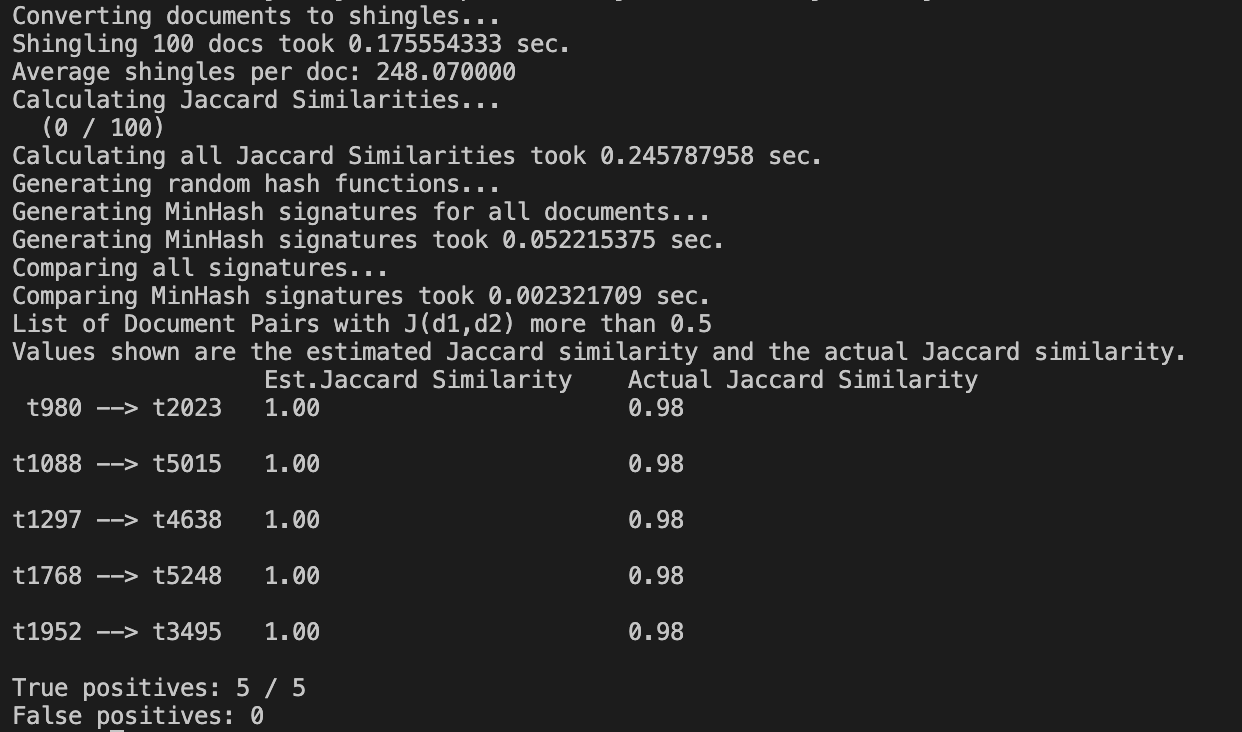
\includegraphics[scale=0.7]{100.png}\\
Input = article\_100.train\\

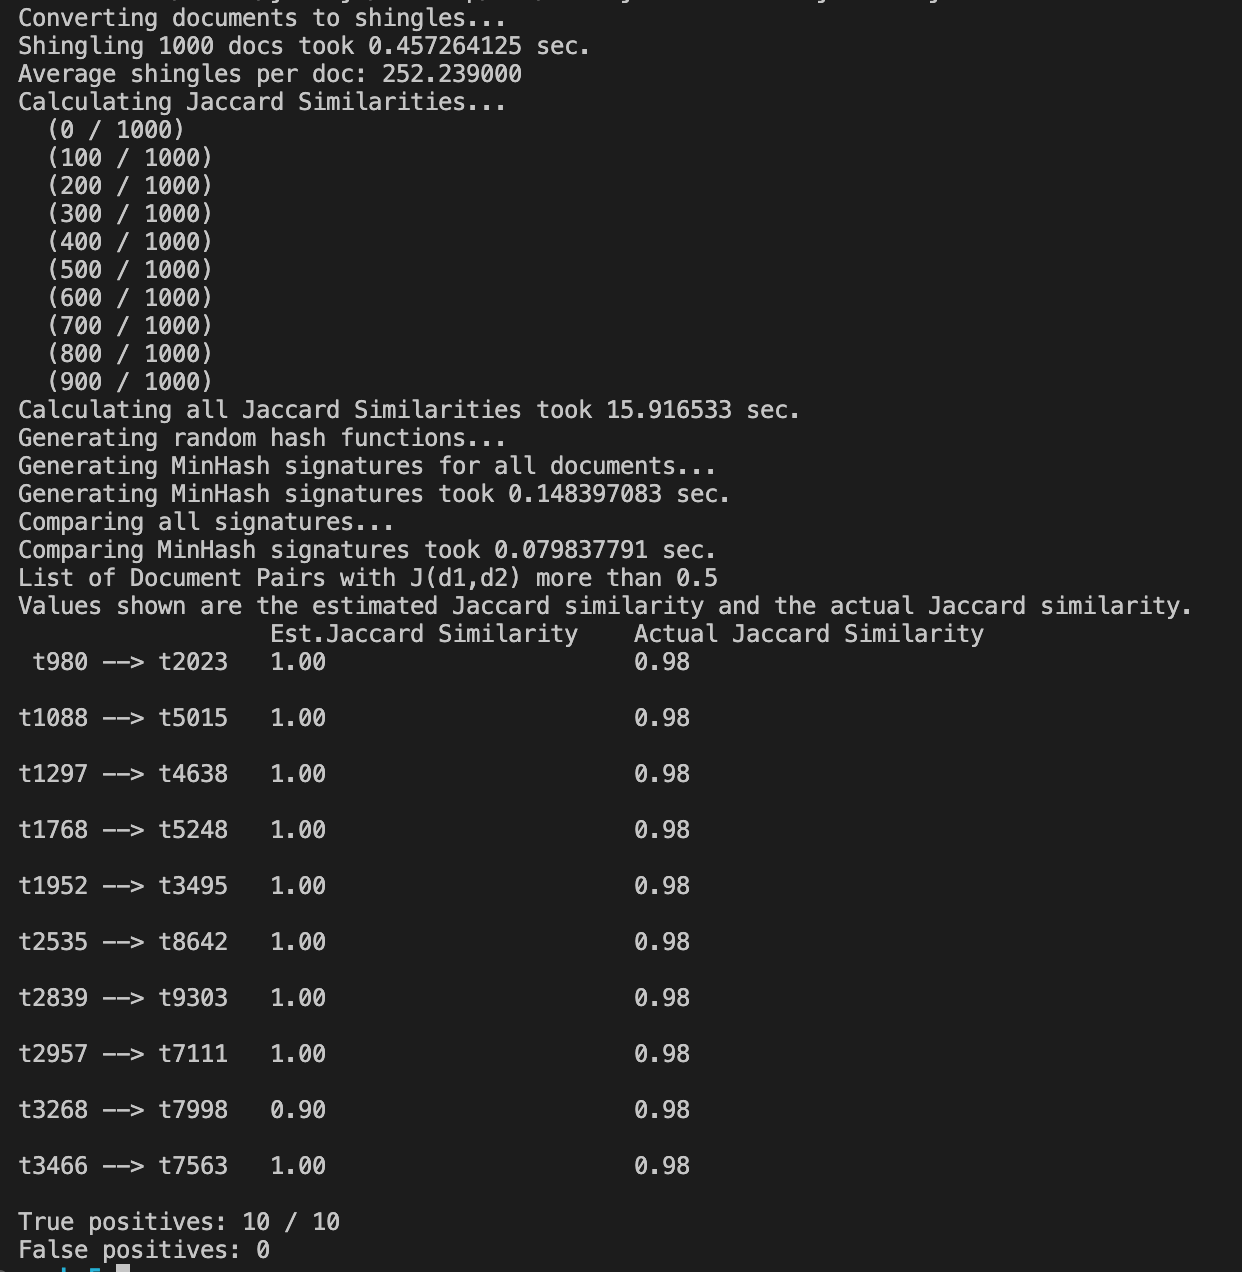
\includegraphics[scale=0.7]{1000.png}\\
Input = article\_1000.train\\

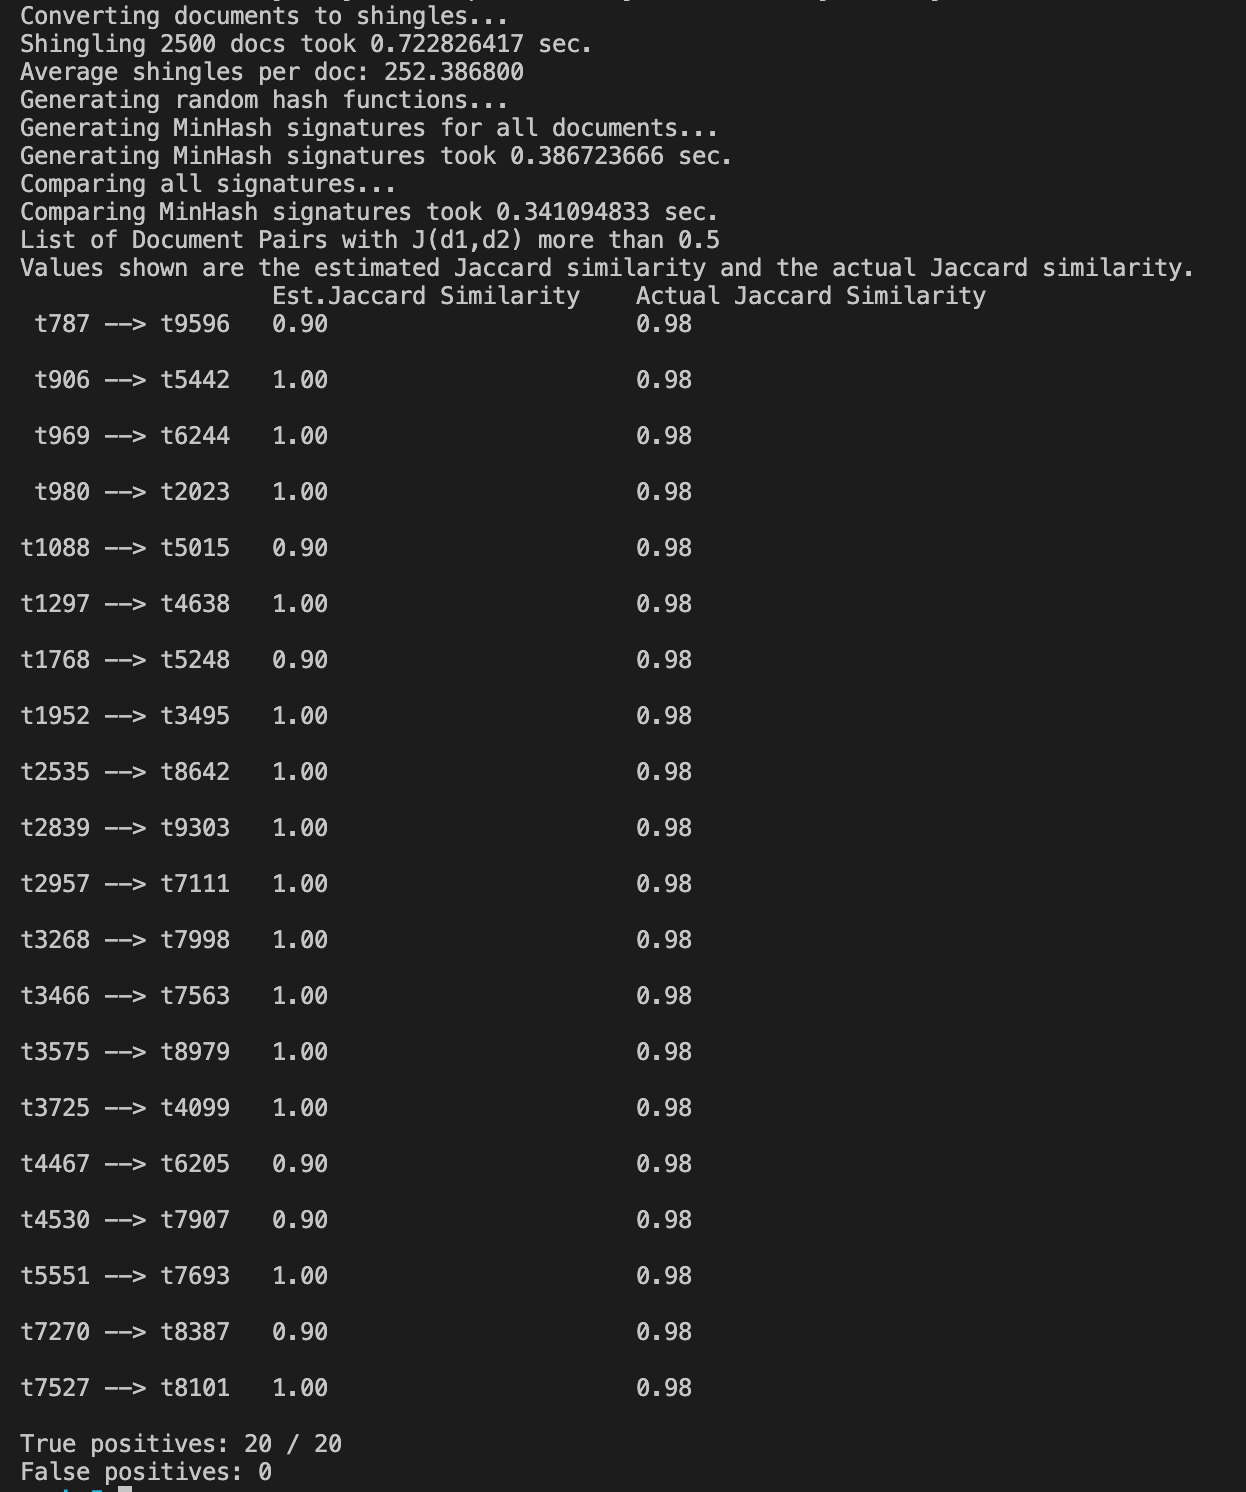
\includegraphics[scale=0.7]{2500.png}\\
Input = article\_2500.train \\

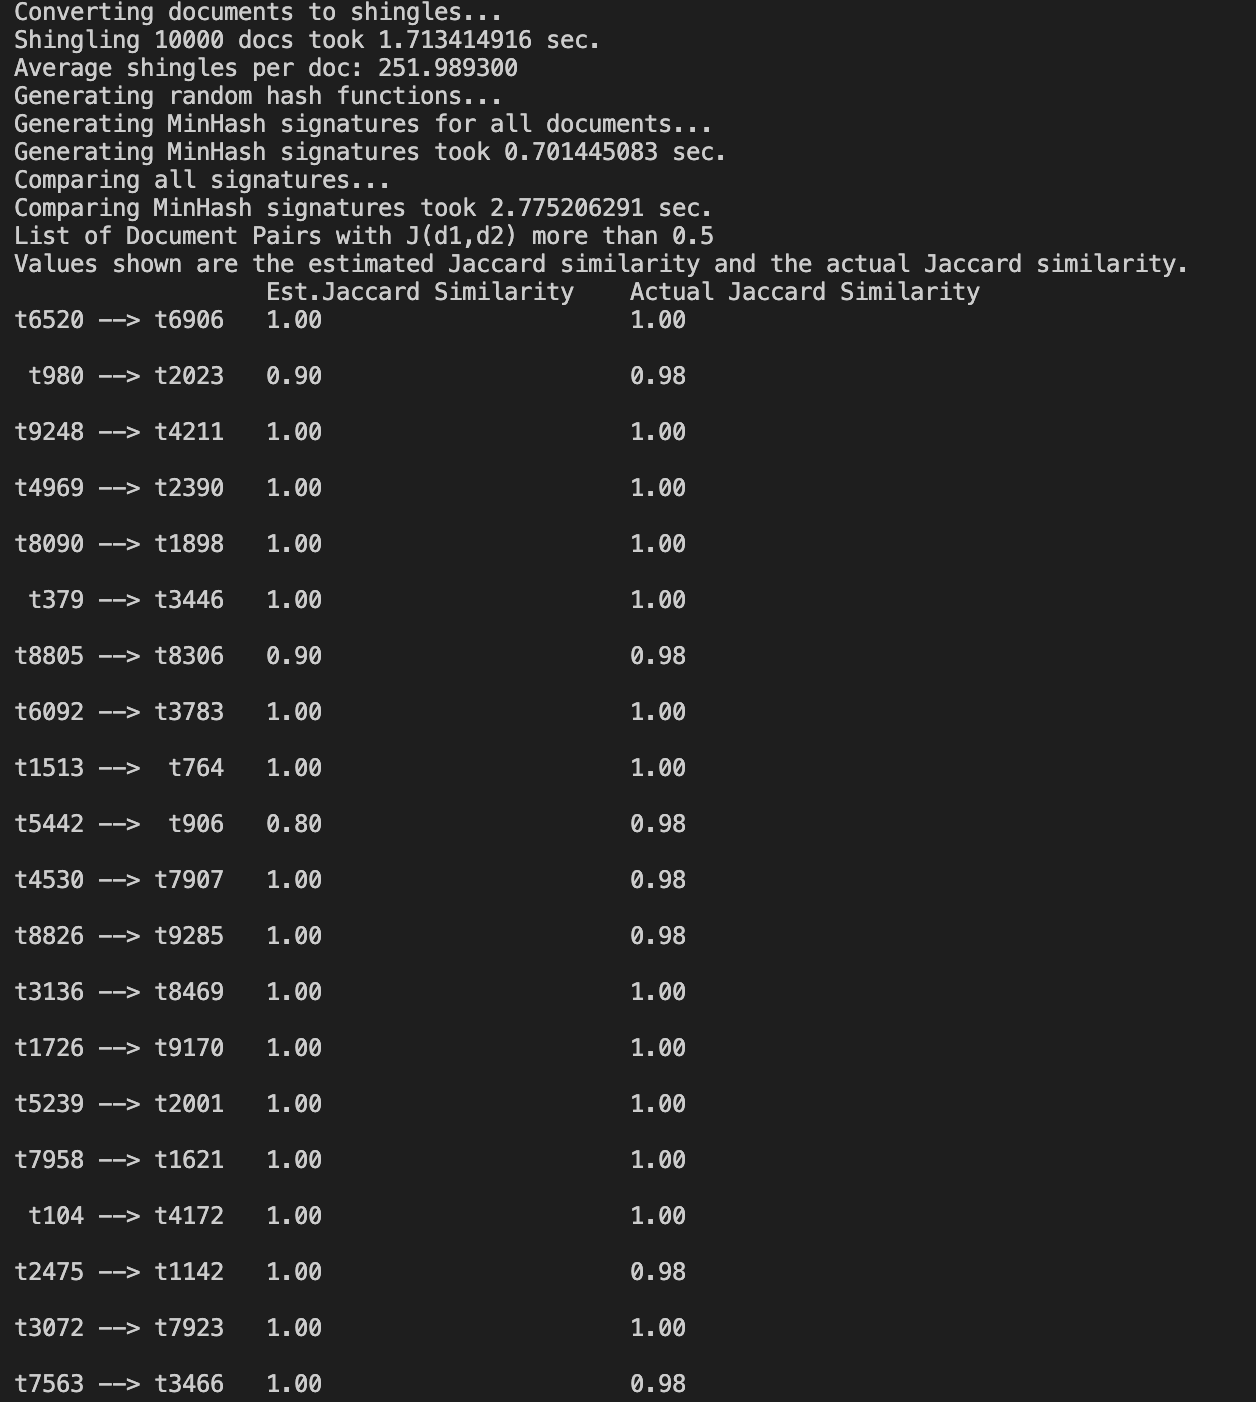
\includegraphics[scale=0.7]{10000-1.png}\\\\
...Rows omitted...\\\\

\includegraphics[scale=0.7]{10000-2.png}\\
Input = article\_10000.train \\

\end{center}

\section*{Insights and Lessons Learned}
From the experiment results shown above, we can see that my Java minHash algorithm has high accuracy in duplicate detection. For all input files, it produces a perfect true positive rate with no false positive. It also runs very fast, with the longest taking around 3 seconds to compute the Jaccard similarities (estimated). \\\\
When looking at the estimated Jaccard Similarity and the actual Jaccard similarity, we can see that minHash is a good estimation. Most of the estimated score is very close to the actual similarity score, and it helps us accurately classify the duplicates. In addition, if we look at the result of processing article\_1000.train, the computation of actual Jaccard Similarity takes about 15 seconds, while the computation of estimated Jaccard Similarity through minHash only takes about 0.15 seconds. This is a huge improvement in efficiency while maintaining accuracy. \\\\
I also learned a few lessons when converting from Python to Java. For example, some of the packages used by the original Python code are not available in Java. Java doesn't have the binascii package, so I had to use the StandardCharsets package to hash shingles to 32-byte integers. I chose this package because it is a standardized way of converting a String to an array of bytes. Intersection and union are also implemented differently in Java compared to Python. It involves creating two additional variables to store the intersection and union of two sets. It seems that Python is more powerful and convenient with some operations, and offers more sophisticated libraries that are easier to use than Java. In addition, I initially used ArrayList of Double objects to store the data, which resulted in running out of Java heap memory. I then changed to arrays with doubles and fixed the issue. We need to consider how the data is stored when translating code that deals with large data.
\end{document}

